% =====================================================================
%  SECTION 8 — Limits: where the certificates stop being useful
%  Draft 1. Every number traceable to RESULTS.md.
% =====================================================================

\section{Limits: contrast, morphology, and the failure mechanism}
\label{sec:limits}

A certificate that is valid but as wide as the analytic envelope conveys
nothing. This section maps where the intervals are useful and where they
are not. We report the unfavourable cases in full: the existing
per-instance neural work is demonstrated at a single contrast
ratio~\cite{Gaynutdinova2026}, and the classical guaranteed-bounds
literature explicitly avoids the high-contrast
regime~\cite{Gaynutdinova2023}, so the boundary of applicability is itself
an open question rather than a matter to be presented favourably.

The morphology classes are shown in Figure~\ref{fig:microstructures}.
All entries below are exact-integration certificates, and all carry the
quality gate of Section~\ref{sec:quad:gate}, so a wide interval can be
attributed either to a genuinely hard problem or to a rejected run.

\begin{figure}[t]
\centering
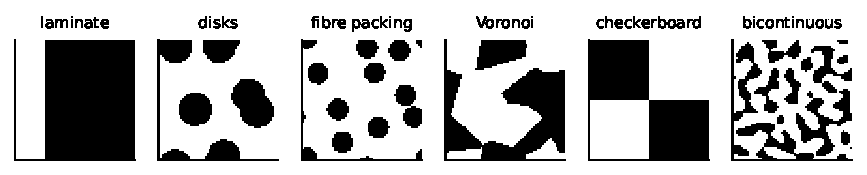
\includegraphics[width=\linewidth]{figures/fig_microstructures.pdf}
\caption{The morphology classes studied, shown at the resolution used for
certification. Left to right: rank-one laminate, overlapping disks,
non-overlapping fibre packing, Voronoi polycrystal, two-phase
checkerboard, and a bicontinuous morphology generated as the level set of a
band-pass filtered Gaussian field.}
\label{fig:microstructures}
\end{figure}

\subsection{Contrast and morphology}
\label{sec:limits:map}

\begin{table}[t]
\centering
\caption{Certified relative width against phase contrast and morphology,
scalar conductivity, $n_q = 64$, $200$ steps. Every entry passed the
quality gate and every certificate was valid. Tightening relative to the
Voigt--Reuss envelope in parentheses.}
\label{tab:map:scalar}
\resizebox{\textwidth}{!}{%
\begin{tabular}{rlll}
\toprule
contrast & disks & laminate & checkerboard \\
\midrule
 10 & 12.4\% (7.5$\times$) & \phantom{0}2.1\% (40.7$\times$) & \phantom{0}19.3\% (5.2$\times$) \\
 50 & 31.8\% (5.3$\times$) & \phantom{0}5.2\% (31.2$\times$) & \phantom{0}88.7\% (1.9$\times$) \\
100 & 44.1\% (4.1$\times$) & \phantom{0}7.4\% (24.5$\times$) &          125.3\% (1.5$\times$) \\
200 & 61.1\% (3.1$\times$) & \phantom{0}9.9\% (19.2$\times$) &          155.3\% (1.2$\times$) \\
\bottomrule
\end{tabular}}
\end{table}

Figure~\ref{fig:map} shows both physics at matched budget. Two
conclusions follow immediately from Table~\ref{tab:map:scalar}.
Morphology dominates contrast: at $200{:}1$ the laminate certificate is
still $9.9\%$ wide and nineteen times tighter than the envelope, while the
checkerboard is $155.3\%$ wide and only $1.2$ times tighter: barely better than a bound computable in closed form from the phase
fractions alone. Reporting certified tightness against contrast alone,
which is the convention in this literature, is therefore misleading; the
useful statement is two-dimensional.

Seeding confirms the map is not an artefact of a fortunate initialisation.
Three seeds per cell at a reduced budget gave, at contrast $10$, widths of
$14.2\%$ (range $13.7$--$14.9\%$) for disks, $3.0\%$ ($2.9$--$3.2\%$) for
the laminate, and $23.0\%$ ($22.9$--$24.0\%$) for the checkerboard; at
contrast $200$, $86.0\%$ ($79.3$--$92.8\%$), $15.0\%$ ($13.6$--$15.8\%$)
and $161.2\%$ ($161.2$--$161.9\%$). Every cell was gate-accepted on every
seed.

\subsection{The same map in elasticity}
\label{sec:limits:elastic}

\begin{table}[t]
\centering
\caption{Certified relative width, controlled synthetic plane-strain elasticity, $n_q = 32$,
$120$ steps. The starred entry failed the quality gate
($\rho = 1.075$); the certificate remains valid but the number reflects a
rejected run.}
\label{tab:map:elastic}
\resizebox{\textwidth}{!}{%
\begin{tabular}{rlll}
\toprule
contrast & disks & laminate & checkerboard \\
\midrule
 10 & 16.3\% (5.0$\times$) & \phantom{0}5.4\% (14.2$\times$) & \phantom{0}28.1\% (3.2$\times$) \\
 50 & 40.3\% (4.0$\times$) &          18.9\% (8.4$\times$)  &          101.1\% (1.6$\times$) \\
200 & 68.8\%$^{*}$ (2.8$\times$) & 63.5\% (3.0$\times$) &          161.8\% (1.2$\times$) \\
\bottomrule
\end{tabular}}
\end{table}

Table~\ref{tab:map:elastic} repeats the controlled synthetic sweep in
elasticity. Within this generated family, the morphology ordering transfers.
At contrast $200$, however, elasticity degrades across \emph{all}
morphologies, including the laminate that remained excellent in the scalar
case. This is evidence about this controlled model family, not an
elastic-material validation result.


\begin{figure}[t]
\centering
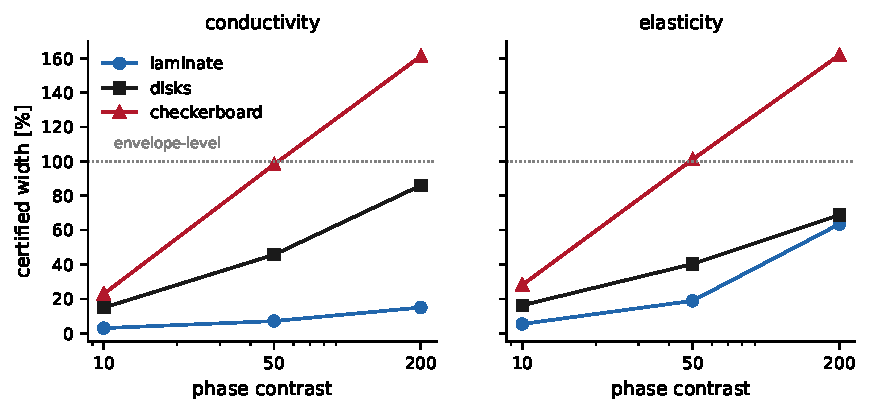
\includegraphics[width=\linewidth]{figures/fig_map.pdf}
\caption{Certified width against phase contrast for three controlled synthetic morphologies, both physics, at matched optimisation budget. The observed morphology ordering is identical in the two panels for this experiment.}
\label{fig:map}
\end{figure}

\subsection{The mechanism is approximation, not physics}
\label{sec:limits:mechanism}

For the controlled generated suite, the ordering laminate $\ll$ disks
$\ll$ checkerboard is consistent with the regularity of the exact
corrector: piecewise linear for the laminate, smooth but curved for
inclusions, and corner-singular for the checkerboard, where four phase
regions meet at a point. The observed widths are consistent with smooth
networks representing singular fields poorly; every entry above was
gate-accepted. This supports an approximation-theoretic explanation for
these numerical cases, rather than a failure of the certification machinery
or a general conclusion about elastic materials.

Figure~\ref{fig:correctors} makes the argument visible: the trained
corrector gradient is uniform in the laminate, smoothly modulated around
the inclusions, concentrated at the four-phase junctions of the
checkerboard, and structured at every scale in the bicontinuous case, in
the same order as the certified widths.

A matched-budget comparison probes these explanations within the controlled
suite. Evaluating both physics at an identical step count gives, for the
checkerboard, $161.2\%$ (conductivity) against $161.8\%$ (elasticity) at
contrast $200$, and $98.2\%$ against $101.1\%$ at contrast $50$: ratios of
$1.00$ and $1.03$. In this controlled comparison, the matched-budget
results do not support the extra loading modes, Poisson coupling or Airy
second derivatives as the dominant explanation for the observed
checkerboard widths. They are consistent with the approximation of a
singular corrector, but do not establish physics independence in general.

The same comparison also corrects a plausible expectation. At matched
budget the elastic certificates are \emph{narrower} than the scalar ones
for the disk morphology at contrasts $50$ and $200$ (ratios $0.88$ and
$0.80$), and wider only for the laminate, dramatically so at $200{:}1$
(ratio $4.23$). This controlled comparison does not support the intuition
that the harder physics yields uniformly wider bounds. It illustrates why
tightness figures need their optimisation budget stated explicitly.

\begin{figure}[t]
\centering
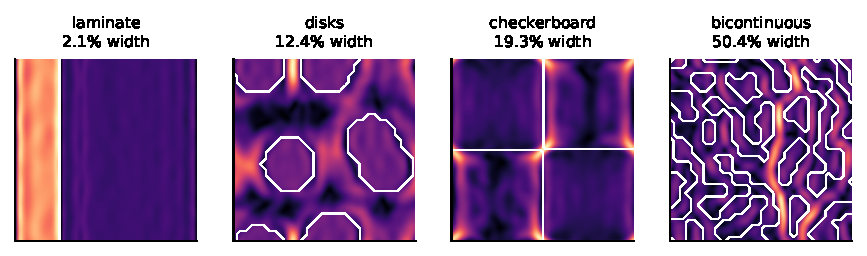
\includegraphics[width=\linewidth]{figures/fig_correctors.pdf}
\caption{Magnitude of the trained corrector gradient for four morphologies
at contrast $10$, with phase boundaries overlaid. Certified width increases
from left to right, tracking the regularity and spatial complexity of the
field rather than any property of the certification scheme.}
\label{fig:correctors}
\end{figure}

\subsection{Realistic morphologies}
\label{sec:limits:realistic}

The microstructures above are idealised. Table~\ref{tab:realistic} repeats
the measurement for three standard models from the composites literature: a
non-overlapping random sequential adsorption fibre packing, a periodic
Voronoi polycrystal, and a bicontinuous morphology generated as the level
set of a band-pass filtered Gaussian field.

\begin{table}[t]
\centering
\caption{Certified width for realistic morphologies, scalar conductivity,
$n_q = 64$, $120$ steps. All gate-accepted; all certificates bracketed an
independent finite-volume reference.}
\label{tab:realistic}
\resizebox{\textwidth}{!}{%
\begin{tabular}{lrr}
\toprule
morphology & contrast $10$ & contrast $50$ \\
\midrule
overlapping disks (baseline) & 14.9\% & \phantom{0}48.8\% \\
fibre packing (RSA)          & 16.7\% & \phantom{0}43.1\% \\
Voronoi polycrystal          & 16.5\% & \phantom{0}56.7\% \\
\textbf{bicontinuous (spinodal)} & \textbf{50.4\%} & \textbf{129.5\%} \\
\bottomrule
\end{tabular}}
\end{table}

Fibre packings and polycrystals behave like the idealised disks, so the
synthetic results transfer. Notably the Voronoi structure is dense with
three-phase junctions yet performs like smooth inclusions: triple junctions
are not the obstacle, and the checkerboard's four-region corner is a
genuinely harsher singularity rather than a generic grain-boundary effect.

The bicontinuous morphology is the hardest realistic class, at $50.4\%$
against the disks' $14.9\%$. This matters practically, since it is the
morphology of porous media, aerogels, polymer blends and battery
electrodes. It also refines the mechanism: a spinodal structure has no
corners, so difficulty cannot be attributed to singular junctions alone.
The unifying statement is that difficulty tracks the \emph{complexity of
the corrector field}, which is driven both by singular junctions and by
percolation with tortuous, multi-scale interfaces. A bicontinuous structure has a nontrivial corrector everywhere rather than only near
isolated inclusions.

Part of this difficulty is resolvable, and the criterion of
Section~\ref{sec:quadrature} prescribes how. The generating field has a
dominant wavenumber of six, while the default embedding resolves only four:
the trial space cannot represent the microstructure's own length scale.
Enriching the embedding to twelve harmonics while simultaneously raising
$n_q$ to maintain headroom reduces the certified width from $50.4\%$ to
$33.2\%$ (Table~\ref{tab:prescription}). The remaining gap to the disk
baseline is genuine.

\subsection{A real segmented micrograph}
\label{sec:limits:micrograph}

The microstructures above are generated. As a final check we take a
published segmented micrograph, use its binary image directly as the
microstructure geometry, and certify the resulting idealised problem. No
measured property is used and no claim is made about the physical
specimen: what is tested is whether the method operates on genuine geometry, with rough interfaces, clustering and percolating veins, rather than on
procedurally generated shapes.

\begin{table}[t]
\centering
\caption{Certifying a real segmented micrograph ($32\times32$ crop, phase
fraction $0.802$, nominal contrast $10$). References: FV $6.0477$, FFT
$6.8094$; Voigt--Reuss width $78.3\%$. The quality gate rejects the two
coarser runs, and the accepted certificate is slightly wider than the
rejected one it replaces.}
\label{tab:micrograph}
\resizebox{\textwidth}{!}{%
\begin{tabular}{rrrrlrrl}
\toprule
$n_q$ & width & tightening & headroom & gate & $K_{\mathrm{low}}$ & $K_{\mathrm{up}}$ & brackets \\
\midrule
 32 & 58.6\% & 1.3$\times$ & 0.87 & reject & 5.5457 & 7.6734 & yes \\
 64 & 34.6\% & 2.3$\times$ & 1.83 & reject & 5.4652 & 7.7238 & yes \\
128 & \textbf{36.8\%} & 2.1$\times$ & \textbf{3.72} & \textbf{accept} & 5.3732 & 7.7692 & yes \\
\bottomrule
\end{tabular}}

\end{table}

A second image exposes a requirement that is easy to miss. Its
autocorrelation half-width is four pixels in a $504$-pixel frame, so any
downsampled representation aliases the geometry: on a $64$-grid the
features span half a pixel. Certified there, the image yields widths of
$19.6\%$ and $49.7\%$, but for a microstructure that is not the one
photographed. Taking instead a native-resolution crop, which preserves the
geometry at the cost of field of view, gives a certified width of
$9.6\%$ on a $48\times48$ crop and $10.5\%$ on $64\times64$, both
gate-accepted at headroom near four, and both bracketing finite-volume and
FFT references that now agree with each other to $1.5\%$ rather than
$9.5\%$. Preserving resolution improves the certificate fivefold and the
references with it.

The requirement is therefore that the certification grid resolve the
smallest features, and we find at least three pixels per correlation
half-width to be necessary. That requirement competes directly with
field of view. A certificate computed on an under-resolved image is valid
for the aliased geometry and says nothing about the original, however tight
it appears. We regard this as a modelling decision to be reported rather
than a numerical parameter to be tuned.

Applied consistently, the protocol is stable. Across two independently
supplied micrographs and two windows in each, native-resolution
certification at $48\times48$ gives certified widths between $9.3\%$ and
$9.9\%$, tightening between $7.5$ and $8.6$ times, headroom near four in
every case, and reference solvers inside every interval. The certified
\emph{values} vary considerably more than the certified widths, since $K_{\mathrm{low}}[1,1]$ ranges from $6.16$ to $6.95$ across the four
windows---which is the expected signature of windows smaller than a
representative volume, and is visible precisely because each window carries
its own certificate rather than a single pooled estimate.

Table~\ref{tab:micrograph} is instructive beyond the headline number. The
criterion of Section~\ref{sec:quadrature} rejects the run twice before
accepting it, and the accepted certificate is marginally \emph{wider} than
the rejected one it replaces. This is the same signature seen in the synthetic
prescription study, where the rejected value was flattered by
under-resolved quadrature. Validity never failed: all three certificates,
including both rejected runs, bracket two independent reference solvers.
Treating the crop instead as a mirrored, genuinely periodic cell gives
$60.4\%$ at headroom $3.56$; the mirrored cell is harder because reflection
doubles the domain, and we report the direct convention as primary with the
mirrored value as a sensitivity check, neither being a property of the
specimen. The certified width of roughly $37\%$ places this micrograph
between the inclusion morphologies and the bicontinuous class, consistent
with its appearance as a percolating network of veins through a majority
phase.

\subsection{A representative-volume study}
\label{sec:limits:rve}

Applying the same protocol to a segmented slice of Berea sandstone, the
standard benchmark of the digital rock physics literature, separates two
quantities that an uncertified method necessarily conflates. We certify
three disjoint windows at each of three sizes, at native resolution, with
the pore phase regularised to a finite conductivity rather than treated as
void.

\begin{table}[t]
\centering
\caption{Berea sandstone: certified width and certified value as the
window grows. Three disjoint windows per size, all gate-accepted. Width is
a property of the method and is nearly constant; value is a property of the
window and is not.}
\label{tab:rve}
\resizebox{\textwidth}{!}{%
\begin{tabular}{rrllr}
\toprule
window & corr.\ lengths & certified width & certified $K_{\mathrm{low}}[1,1]$ & spread \\
\midrule
32 & \phantom{0}5 & 12.1\% [8.8, 12.4] & 2.710 [2.011, 3.033] & 1.51$\times$ \\
48 & \phantom{0}8 & \phantom{0}9.5\% [7.9, 14.2] & 4.929 [3.115, 5.317] & 1.71$\times$ \\
64 & 11 & \phantom{0}9.8\% [8.8, 16.4] & 6.069 [4.334, 6.317] & 1.46$\times$ \\
\bottomrule
\end{tabular}}

\end{table}

The certified width is essentially flat at $9$--$12\%$ across a fourfold
change in window area: it reflects how well smooth trial fields represent
this morphology and does not improve with more material. The certified
value, by contrast, more than doubles between windows of five and eleven
correlation lengths and still varies by factors of $1.5$ to $1.7$ between
windows of equal size. This slice is far from representative for
conductivity at these window sizes, notwithstanding that the full image
contains some $166$ correlation lengths.

The decomposition is the contribution. Presented with four different values
from four windows, a point-estimate surrogate cannot attribute the
variation to the material or to itself. Because each window here carries
its own certificate, the $10\%$ is attributable to the method and the
$1.5\times$ to the material, at no additional cost.

\subsection{Scope of the claims}
\label{sec:limits:scope}

Collecting the controlled numerical experiments above, the scalar
conductivity certificates are between three and forty times tighter than the
analytic envelope for the stated layered, particulate, fibrous and
polycrystalline morphologies up to approximately $100{:}1$ contrast. The
generated plane-strain cases provide an internal stress test of the same
construction, but not an externally labelled elasticity coverage study. In
the controlled families, certificates degrade towards the envelope for
corner-singular and bicontinuous morphologies at high contrast. This
identifies a trial-field approximation limitation in the reported numerical
experiments; it does not establish a general material-performance law.
